\documentclass[a4paper, 12pt]{article}
\usepackage[T2A]{fontenc}
\usepackage[utf8]{inputenc}
\usepackage[english,russian]{babel}
\usepackage{titletoc}
\usepackage{graphicx}
\usepackage{array}
\usepackage{etoolbox}
\usepackage{subfig}
\newcolumntype{P}[1]{>{\centering\arraybackslash}p{#1}}
\def\textunderset#1#2{\leavevmode
  \vtop{\offinterlineskip\halign{%
    \hfil##\hfil\cr\strut#2\cr\noalign{\kern-.3ex}
    \hidewidth\strut#1\hidewidth\cr}}}
\def\signhrule{\raggedright\baselineskip30.0ex \vrule height 0.5pt width30mm depth0pt}


\dottedcontents{section}[2.5em]{\bfseries}{2em}{0.5pc}
\dottedcontents{subsection}[3em]{}{2em}{0.5pc}

\usepackage{hyperref}
\hypersetup{
    colorlinks=true, %set true if you want colored links
    linktoc=all,     %set to all if you want both sections and subsections linked
    linkcolor=black,  %choose some color if you want links to stand out
}

\usepackage{verbatim}

\usepackage{listings}
\usepackage{xcolor}

\lstset
{%
	extendedchars=\true,
	inputencoding=utf8x,
	keepspaces=true,
	frame=tb,
	escapechar=|,
	xleftmargin=0.5cm,
	xrightmargin=0.5cm,
	columns=fullflexible,
	numbers=left,
	numbersep=4pt,
	showspaces=false,
	showstringspaces=false,
	breakatwhitespace=true,
	breaklines=true,
	basicstyle=\color{black}\small\sffamily,
	commentstyle=\color{gray}\itshape,
	stringstyle=\color{orange},
	numberstyle=\footnotesize\color{gray},
	keywordstyle=\color{blue}\bfseries,
	emphstyle={\color{blue}\bfseries},
	tabsize=2,
	texcl=true,
}

\lstdefinestyle{text}{
basicstyle=\small\ttfamily,
columns=flexible,
breaklines=true,
breakatwhitespace=true,
literate={\-}{{-\allowbreak}}1,
numbers=none,
postbreak=\mbox{\textcolor{red}{$\hookrightarrow$}\space},
}

\lstloadlanguages{SQL}

\newcommand{\Title}{Отчет о выполнении лабораторной работы}
\newcommand{\TaskType}{лабораторная работа}
\newcommand{\SubTitle}{по дисциплине <<Поддержка принятия решений в системах мониторинга>>}
\newcommand{\LabTitle}{Выявление логических закономерностей по данным мониторинга} 
\newcommand{\Faculty}{<<Информатика и системы управления>>}
\newcommand{\Department}{<<Компьютерные системы и сети (ИУ-6)>>}
\newcommand{\AuthorFull}{Козлов Владимир Михайлович}
\newcommand{\Author}{Козлов В.М.}
\newcommand{\Teacher}{}
\newcommand{\group}{ИУ6-13М}
\newcommand{\Year}{2024}
\newcommand{\Country}{Россия}
\newcommand{\City}{Москва}

\newcommand{\UpperFullOrganisationName}{Министерство науки и высшего образования Российской Федерации}
\newcommand{\ShortOrganisationName}{МГТУ~им.~Н.Э.~Баумана}
\newcommand{\FullOrganisationName}{федеральное государственное бюджетное образовательное учреждение высшего профессионального образования\newline <<Московский государственный технический университет имени Н.Э.~Баумана (национальный исследовательский университет)>> (\ShortOrganisationName)}

\textwidth=163mm
\textheight=220mm
\oddsidemargin=-0.5pt
\footskip=30pt
\topmargin=27pt
\headheight=12pt
\headsep=25pt
\topskip=10pt
\baselineskip=15pt
\topmargin=-4mm
\begin{document}
\vspace*{-\baselineskip}
\vspace*{-\headheight}
\vspace*{-\headsep}
\vspace*{-2pt}
\thispagestyle{empty}
\begin{center}

% Шапка
{\centering
\begin{tabular}{P{0.15\textwidth}P{0.85\textwidth}}
\smash{
		\raisebox{-0.9\height}{
		
\includegraphics[width=0.15\textwidth]{includes/bmstu.pdf}
		}}
 & \UpperFullOrganisationName\newline \FullOrganisationName \\
\hline
\multicolumn{1}{p{0.15\textwidth}}{} & \multicolumn{1}{p{0.85\textwidth}}{} \\
\multicolumn{1}{p{0.15\textwidth}}{ФАКУЛЬТЕТ}	&	\multicolumn{1}{p{0.85\textwidth}}{\Faculty}	\\
\multicolumn{1}{p{0.15\textwidth}}{КАФЕДРА}	&	\multicolumn{1}{p{0.85\textwidth}}{\Department}	\\
\end{tabular}}
\vfil

{% Основная часть
\vfil
\Large
\underline{\MakeUppercase{\Title}}
\newline
\SubTitle
\vfil
\large
\begin{tabular}{p{0.3\textwidth}p{0.5\textwidth}} 
	Студент:	& \AuthorFull \\ 
	\hline
	Группа:	& \group \\ 
	\hline
	Тип задания:	& \TaskType \\ 
	\hline
	Тема:	& \LabTitle \\ 
	\hline
	\end{tabular}

\vfil

\begin{tabular}{p{0.45\textwidth}p{0.25\textwidth}P{0.25\textwidth}} 
\large
Студент	&	\textunderset{\scriptsize{подпись, дата}}{\signhrule} & \textunderset{\scriptsize{Фамилия, И.О.}}{\ifdefempty{\Author}{\signhrule}{\underline{\Author}}} \\ 
& & \\
Преподаватель	&	\textunderset{\scriptsize{подпись, дата}}{\signhrule} & \textunderset{\scriptsize{Фамилия, И.О.}}{\ifdefempty{\Teacher}{\signhrule}{\underline{\Teacher}}} \\ 
\end{tabular}
}

\vfil
\vfil
\City, \Year

\end{center}

\pagebreak
\tableofcontents
\newpage
% Основная часть --------------------------------------------------------------------------------------------
\section*{Цель}
\addcontentsline{toc}{section}{Цель}
Изучение способов выявления закономерностей в разнородных данных.
\section*{Задание}
\addcontentsline{toc}{section}{Задание}
Имеются два класса изображений лиц людей (смотри рисунок 1).
Найти закономерности группирования этих изображений и определить, чем
лица разных классов отличаются друг от друга и что объединяет лица одного
класса.
\begin{center}
  \centering
  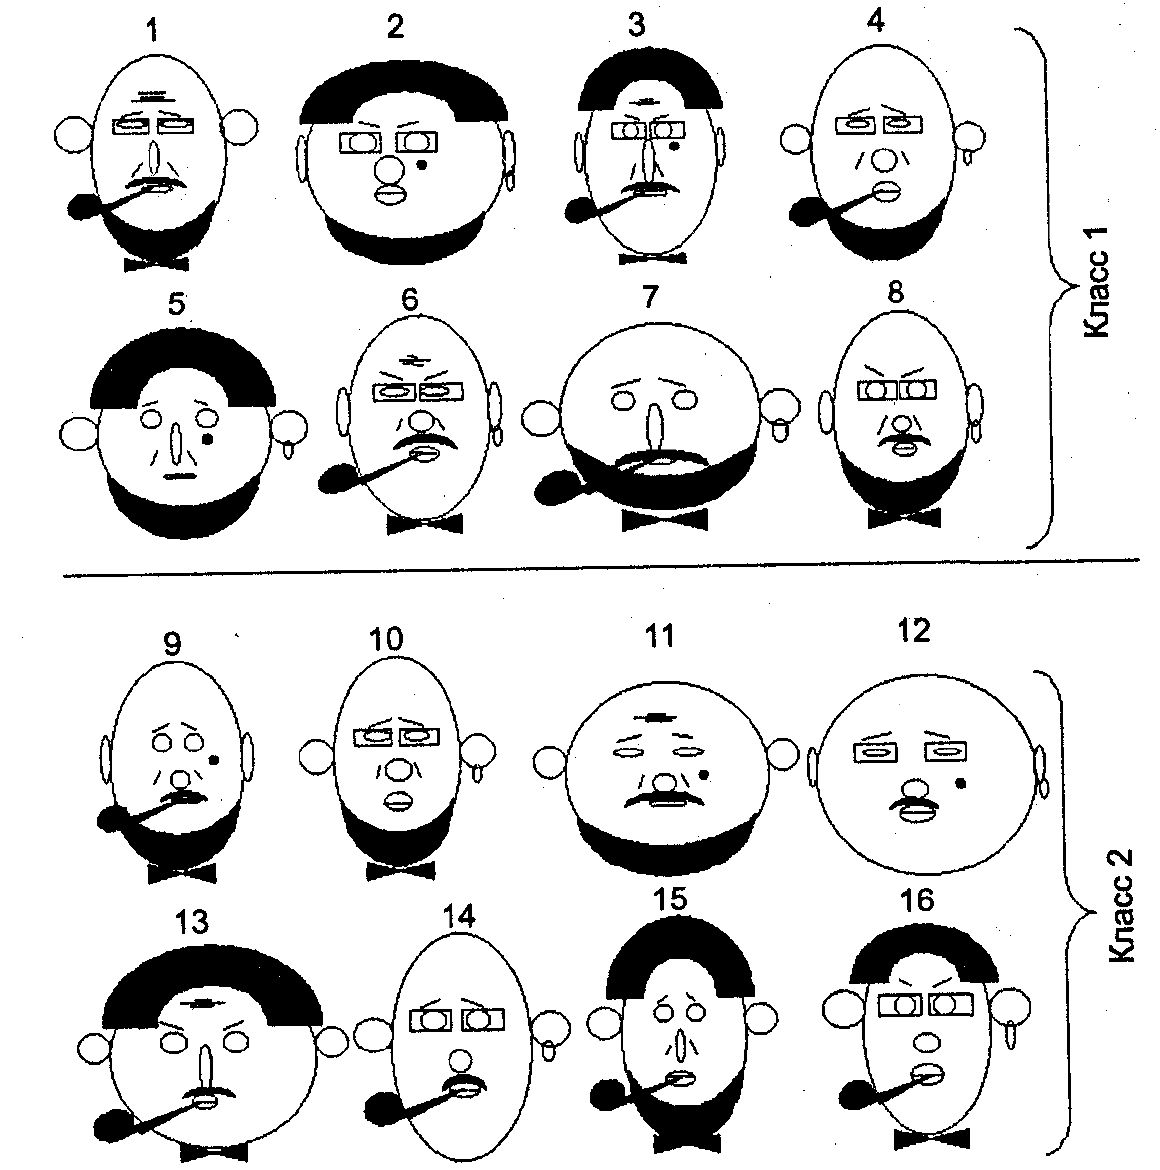
\includegraphics[width=.7\linewidth]{extra/faces.jpg}
  \captionof{figure}{2 класса лиц}
  \label{fig:prplot}
\end{center}
\newpage
% -------------------------------------------------------
\section{Выполнение работы}
\subsection{Признаки и классы}
Были выделены следующие признаки:
\begin{enumerate}
  \item (голова): круглая - 1, овальная - 0;
  \item (уши): оттопыренные - 1, прижатые - 0;
  \item (нос): круглый - 1, длинный - 0;
  \item (глаза): круглые - 1, узкие - 0;
  \item (лоб): с морщинами - 1, без морщин - 0;
  \item (складка): носогубная складка есть - 1, носогубной складки нет - 0;
  \item (губы): толстые - 1, тонкие - 0;
  \item (волосы): есть - 1, нет - 0;
  \item (усы): есть - 1, нет - 0;
  \item (борода): есть - 1, нет - 0;
  \item (очки): есть - 1, нет - 0;
  \item (родинка): родинка на щеке есть - 1, родинки на щеке нет - 0;
  \item (бабочка): есть - 1, нет - 0;
  \item (брови): подняты кверху - 1, опущены книзу - 0;
  \item (серьга): есть - 1, нет - 0;
  \item (трубка): курительная трубка есть - 1, нет - \item
\end{enumerate}
Так как выделение закономерностей вполнено на языке Python, то и данные заносятся на нём. На следующем листинге можно увидеть массив элементов с кортежем из массива признаков и класса, к оторому принадлежит элемент.
\lstinputlisting[language=Python, caption=Признаки и классы]{../data.py}
Для решения используется наивный байессовкий классификатор. На следующем листинге представлен код классификатора.
\lstinputlisting[language=Python, caption=Код классификатора]{../bayes.py}
Для проверки адекватности проводилась следующим кодом:
\lstinputlisting[language=Python, caption=Проверка адекватности]{../main.py}
\textbf{Результат:} Ошибка в 5 случев из 8 \\
\textbf{Вывод:} В силу малого количества данных байесовкий классификатор не даёт хороших результатов. Также формула не срабатывет корректно если в классе у всех элементов совпадает признак так как в таком случае он бессмысленнен.
\newpage
% -------------------------------------------------------
\section{Ответы на вопросы}
\subsection*{Вопросы}
\begin{enumerate}
  \item Что понимается под закономерностями в данных? Приведите промеры типовых закономерностей;
  \item Поясните основные подходы выявления и анализа закономерностей внутри данных;
  \item Укажите и поясните основные статистические методы для выявления закономерностей в данных;
  \item Укажите интеллектуальные методы, применяемые для анализа больших данных;
  \item С какой целью проводится кодирование информационных признаков?
  \item Как можно определить логические закономерности в данных?
  \item С какой целью проводится предварительная обработка данных при мониторинге? Что она включает?
\end{enumerate}
\subsection*{Ответы}
\begin{enumerate}
  \item Закономерности в данных — это повторяющиеся шаблоны или тенденции, которые можно обнаружить в наборе данных. Они помогают понять, как различные переменные взаимодействуют друг с другом и могут быть использованы для прогнозирования будущих значений или поведения.\\
  Вот несколько примеров типовых закономерностей:
  \begin{enumerate}
    \item Линейные
    \item Сезонные
  \end{enumerate}
  \item \begin{enumerate}
    \item Статистический анализ - определение взаимосвязей исходя из статистики через основные характеристики и коэффициенты корреляции.
    \item Визуализация данных - визуализация данных в виде различных графиков или тепловых карт.
    \item Машинное обучение - разделение данных исходя из признаков путём классификации, регрессии или кластеризации.
    \item Анализ временных рядов -  Используется для выявления закономерностей в данных, собранных во времени.
  \end{enumerate}
  \item Основные статистические методы:
  \begin{enumerate}
    \item Описательная статистика.
    \item Корреляционный анализ.
    \item Регрессионный анализ.
    \item Кластерный анализ.
    \item Факторный анализ.
  \end{enumerate}
  \item \begin{enumerate}
    \item машинное обучение;
    \item дата майнинг;
    \item нейросети;
    \item имитационные модели;
    \item предикативный и статистический анализ.
  \end{enumerate}
  \item Чтобы можно было представить информацию в формате матрицы
  0 и 1, и использовать её для математической обработки с помощью
  машинного обучения по средством написания кода. Или для простого
  более наглядного, упорядоченного представления информации.
  \item Полученную информацию можно представить графически,
  использовать графы или закодировать и отсортировать в таблице. После
  чего либо ручным анализом (например деревья), либо с помощью
  компьютерных программ, выявляющим закономерности в
  закодированной информации.
  \item Предварительная обработка данных при мониторинге проводится с целью улучшения качества данных и повышения точности анализа. Она включает в себя несколько ключевых этапов: 
  \begin{enumerate}
    \item Очистка данных.
    \item Нормализация.
    \item Трансформация.
    \item Отбор признаков.
    \item Заполнение пропусков.
    \item Агрегация.
  \end{enumerate}
\end{enumerate}
\newpage
%---------------------------------------------------------
\section{Вывод}
в результате данной лабораторной работы был проведен
системный анализ данных, изучены различные способы выявления
закономерностей в данных и реализован один из них.
\end{document}
